\documentclass[aspectratio=169]{beamer}
\usepackage{tikz}
\usepackage{graphicx}
\usepackage{xypic}
\usepackage[table]{xcolor}

\usecolortheme{whale}
\usetikzlibrary{er,positioning}  
\usetikzlibrary{decorations.pathreplacing}
\usetikzlibrary{arrows, decorations.markings}
\usetikzlibrary{shapes.geometric}
\usetikzlibrary{mindmap}

\setbeamertemplate{navigation symbols}{}

% \setbeameroption{show notes on second screen=right}

\definecolor{violet}{rgb}{0.53, 0.0, 0.69}

\definecolor{blue1}{RGB}{126,126,206}
\definecolor{blue2}{RGB}{87,87,192}
\definecolor{blue3}{RGB}{51,51,178}
\definecolor{blue4}{RGB}{27,26,107}
\definecolor{red1}{RGB}{237,146,124}
\definecolor{green1}{RGB}{208,235,201}

\tikzstyle{every link} = []
\tikzstyle{link} = [>=triangle 60, draw, every link]

\definecolor{attr}{RGB}{10,153,2}

\graphicspath{{img/}{./}} % Specifies where to look for included images (trailing slash required)

\newcommand<>{\red}[1]{\textcolor#2{red}{#1}}
\newcommand<>{\green}[1]{\textcolor#2{green}{#1}}
\newcommand<>{\gray}[1]{\textcolor#2{gray}{#1}}


\title{Bases de Datos Orientadas a Grafos}
\subtitle{}
\author[Garc\'ia L., Cardentey V. M., Ledesma. A]{
    Lic. Andy Ledesma Garc\'ia\\ 
    Lic. V\'ictor M. Cardentey Fundora\\ 
    Dra. C. Lucina Garc\'ia Hern\'andez
}
\institute[MATCOM-UH]{
    Departamento de Computaci\'on\\
    Facultad de Matem\'atica y Computaci\'on\\
    Universidad de La Habana\\[3mm]
    Licenciatura en Ciencia de Datos
}
\date[]{6 de febrero de 2025}


\begin{document}
    \maketitle
    % \section{Objetivos}
    % \input{objectives.tex}

    \begin{frame}
    \frametitle{Modelo de datos}

    \begin{block}{Estructura de datos}
        Un grafo $G = <V,E>$ es una par formado por dos conjuntos
        $V$ y $E$, donde $V$ es un conjunto finito, cuyos elementos representan
        los vértices (o nodos) del grafo y $E$ es un conjunto de pares
        de elementos de $V$, a los cuales se les llama aristas, estos pares pueden ser ordenados o no ordenados.

        \centering
        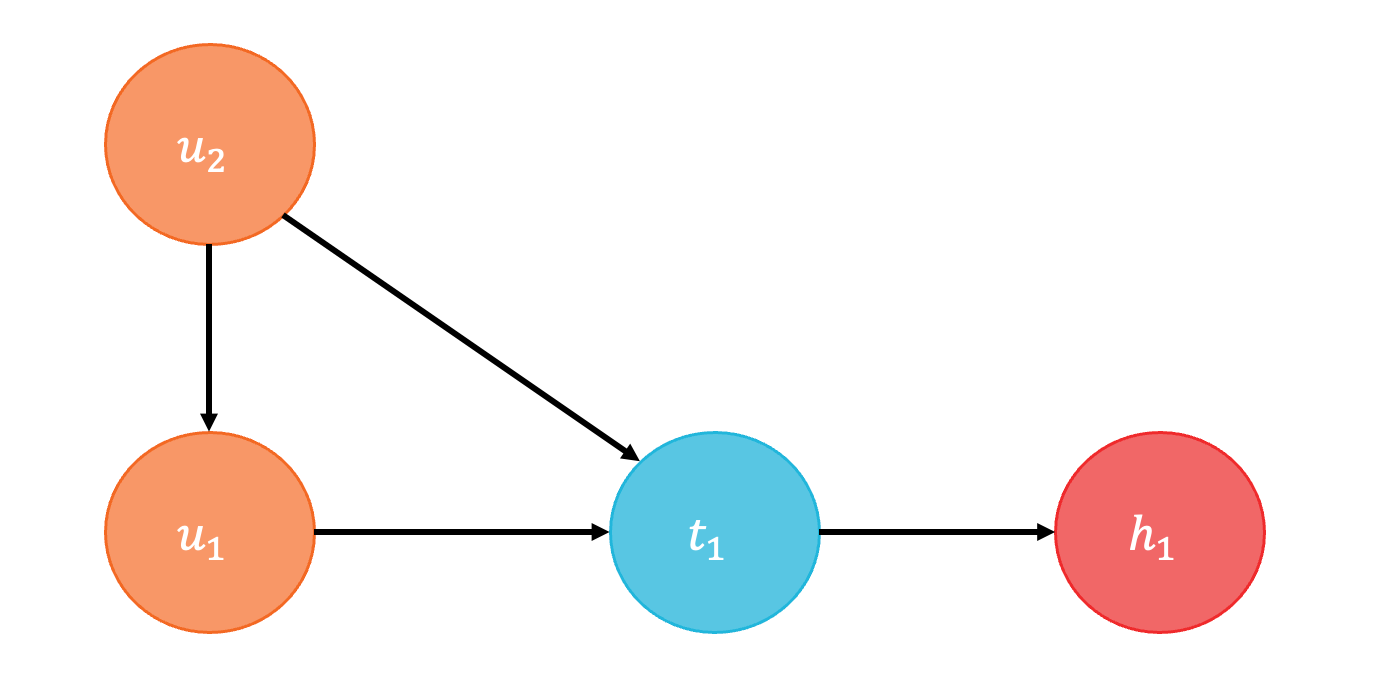
\includegraphics[width=0.6\textwidth]{img/base-graph.png}


    \end{block}
\end{frame}

\begin{frame}
    \frametitle{Modelo de datos}

    \begin{block}{Estructura de datos}
        Un grafo etiquetado $G_e = <G,I,T>$ es una terna de elementos, 
        donde $G$ es un grafo, $T$ es un conjunto de etiquetas
        e $I$ es una función $I: G(V) \cup G(E) \to 2^T$ que asigna las etiquetas a los vértices y aristas del grafo.

        \centering
        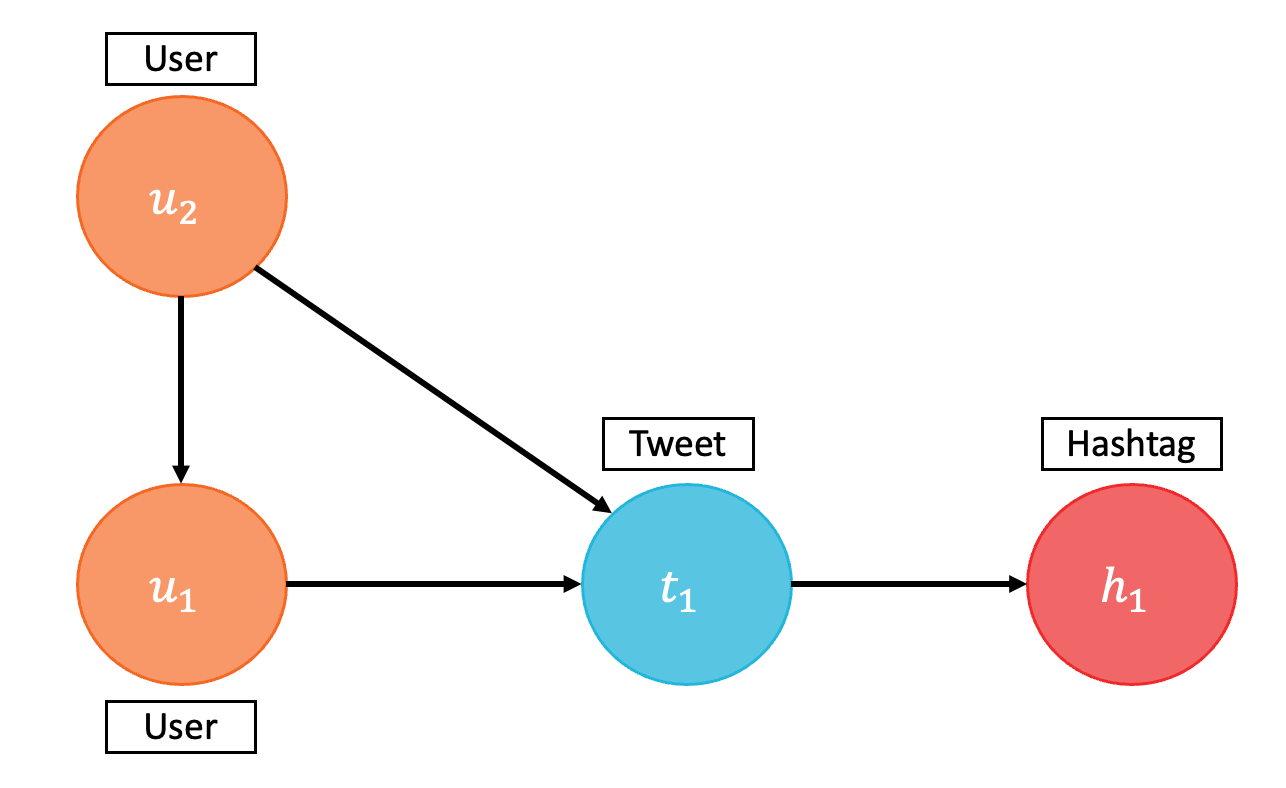
\includegraphics[width=0.6\textwidth]{img/labeled-graph.png}


    \end{block}
\end{frame}

\begin{frame}
    \frametitle{Modelo de datos}

    \begin{block}{Estructura de datos}
        Un grafo atributado $G_a = <G,I,A>$ es una terna de elementos, 
        donde $G$ es un grafo, $A$ es un conjunto de atributos
        e $I$ es una función $I: G(V) \cup G(E) \to 2^A$ que asigna los atributos a los vértices y aristas del grafo.

        \centering
        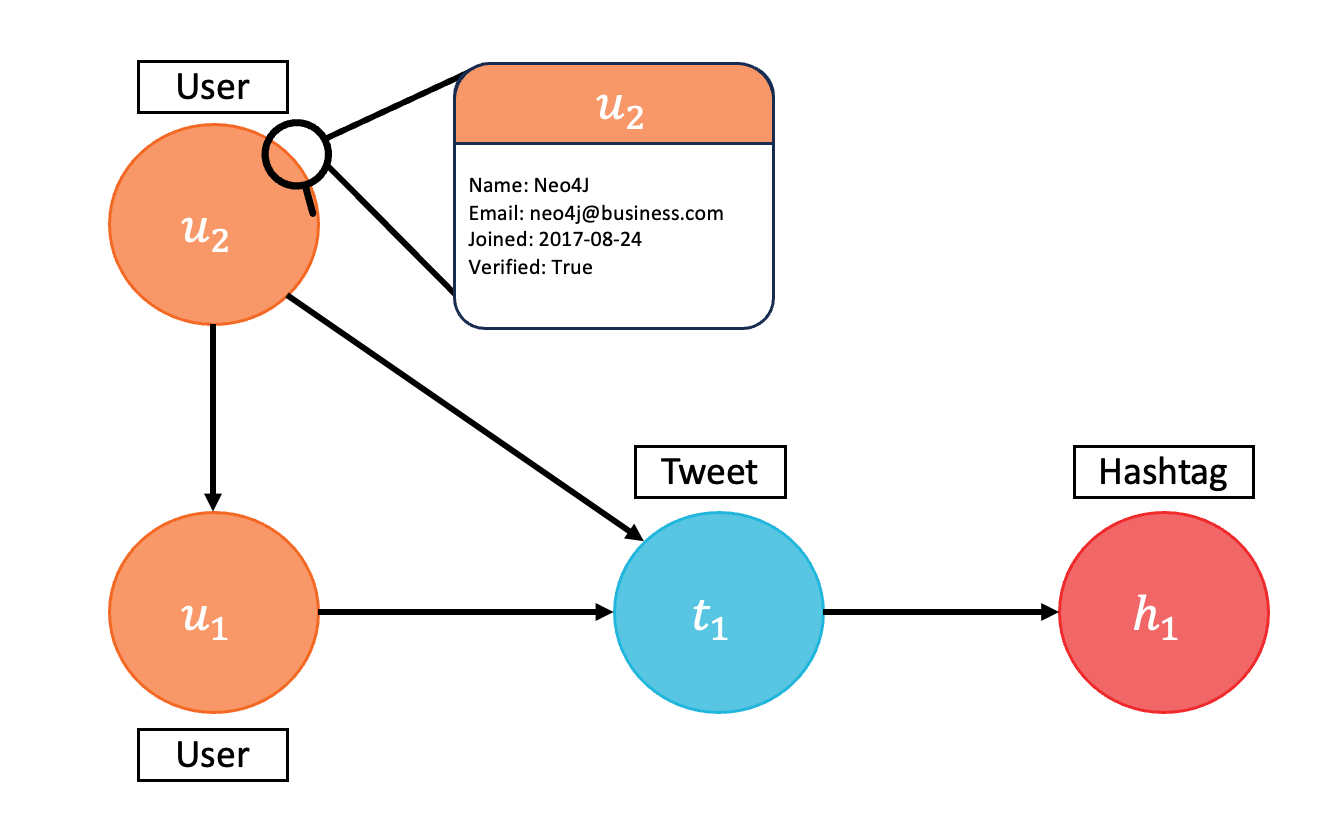
\includegraphics[width=0.6\textwidth]{img/attributed-graph.png}


    \end{block}
\end{frame}

\begin{frame}
    \frametitle{Modelo de datos}

    \begin{block}{Restricciones de integridad}
        \begin{itemize}
            \item Las llaves de los vértices deben ser un \texttt{string} que debe ser único dentro del vértice
            \item El valor de una misma llave puede ser de distintos tipos de datos
            \item Integridad referencial
        \end{itemize}

    \end{block}

    \note<1>{@NOTE x ejemplo:
        \begin{itemize}
            \item referenciar a valores \'unicos
            \item eliminar redundancia en datos repetidos continuamente (Run-Length Encoding)
            \item eliminaci\'on de nulls llevando m\'ascaras de bits, por ejemplo
        \end{itemize}
    }
\end{frame}

\begin{frame}
    \frametitle{Modelo de datos}

    \begin{block}{Operaciones}
        \begin{itemize}
            \item Operaciones CRUD básicas
            \item Recorrido de grafos
            \item La complejidad de las operaciones de consulta dependen del sistema gestor ya que no existe un estándar para
            estas bases de datos. Generalmente incluyen operadores análogos a los de SQL.
        \end{itemize}

    
    \end{block}

    \note<1>{@NOTE x ejemplo:
        \begin{itemize}
            \item referenciar a valores \'unicos
            \item eliminar redundancia en datos repetidos continuamente (Run-Length Encoding)
            \item eliminaci\'on de nulls llevando m\'ascaras de bits, por ejemplo
        \end{itemize}
    }
\end{frame}

% \begin{frame}
%     \frametitle{Consideraciones}

%     \begin{table}[h!]
%         \centering
%         \begin{tabular}{|p{0.45\textwidth}|p{0.45\textwidth}|}
%         \hline
%         \multicolumn{1}{|c|}{\cellcolor{green1} \textbf{Ventajas}} &  \multicolumn{1}{|c|}{ \cellcolor{red1} \textbf{Desventajas}} \\ \hline
%         El modelo de datos de documento es ampliamente utilizado en la programación permitiendo
%         una comunicación más directa entre la base de dato y las aplicaciones & Carencia de un estándar para la interacción con este modelo \\ \hline
%         Flexibilidad para la modelación de datos permitiendo incluso implementar un modelo relacional & No se asegura el cumplimiento de reglas de negocio \\ \hline
%         Gran disponibilidad y escalabilidad & No cumple con ACID \\ \hline
%         \end{tabular}
%     \end{table}

%     % \note<2>{@NOTE x ejemplo:
%     %     \begin{itemize}
%     %         \item referenciar a valores \'unicos
%     %         \item eliminar redundancia en datos repetidos continuamente (Run-Length Encoding)
%     %         \item eliminaci\'on de nulls llevando m\'ascaras de bits, por ejemplo
%     %     \end{itemize}
%     % }
% \end{frame}


\begin{frame}
    \frametitle{Casos de uso}

   Se utilizan en escenarios que pueden modelarse como una red compleja

    \begin{itemize}
        \item Redes sociales
        \item Detección de fraude en redes bancarias
        \item Modelación de redes en bioinformática
    \end{itemize}

    % \note<2>{@NOTE x ejemplo:
    %     \begin{itemize}
    %         \item referenciar a valores \'unicos
    %         \item eliminar redundancia en datos repetidos continuamente (Run-Length Encoding)
    %         \item eliminaci\'on de nulls llevando m\'ascaras de bits, por ejemplo
    %     \end{itemize}
    % }
\end{frame}



\begin{frame}
    \frametitle{Implementación de un caso de uso}

    
    \begin{block}{Descripción}
        X (anteriormente Twitter) es una red social donde los usuarios pueden compartir mensajes cortos llamados posts (tweets). Permite publicar textos, imágenes, videos y enlaces, así como interactuar con otros usuarios a través de respuestas, reposts (retweets) y "me gusta".

    \end{block}
    % \note<2>{@NOTE x ejemplo:
    %     \begin{itemize}
    %         \item referenciar a valores \'unicos
    %         \item eliminar redundancia en datos repetidos continuamente (Run-Length Encoding)
    %         \item eliminaci\'on de nulls llevando m\'ascaras de bits, por ejemplo
    %     \end{itemize}
    % }

    \begin{center}
        
        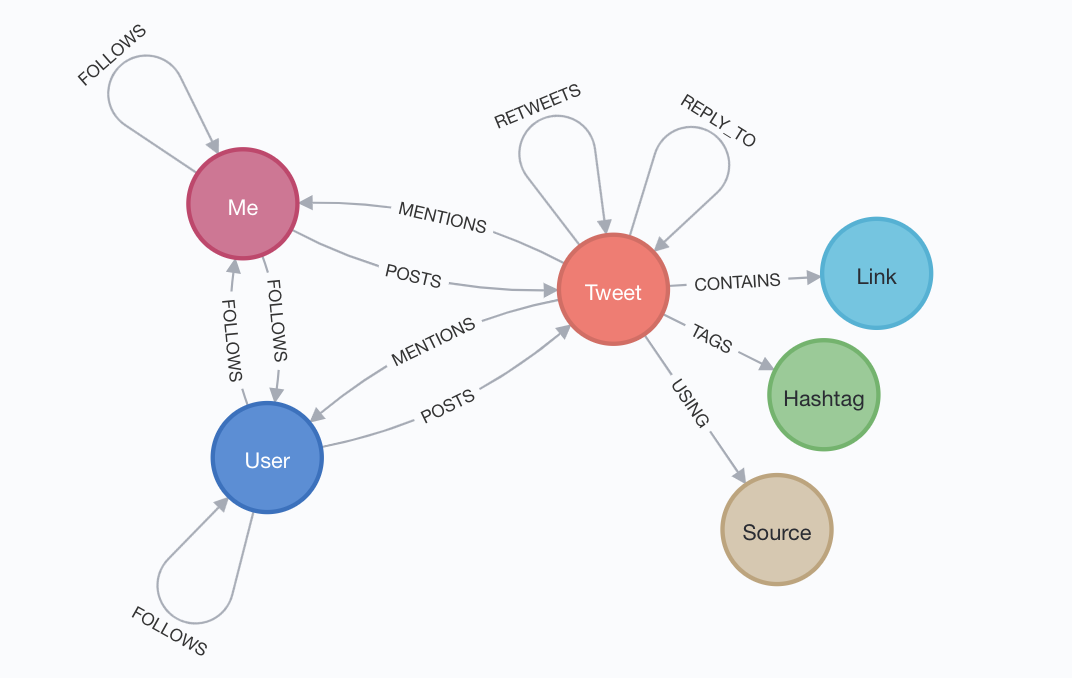
\includegraphics[width=0.5\textwidth]{img/model.png}
    \end{center}
\end{frame}



% \begin{frame}
%     \frametitle{Implementación de un caso de uso}

%     \begin{block}{Requerimientos}
%         \begin{itemize}
%             \item \textbf{Simplicidad conceptual}: Solo es necesario almacenar los nombres de dominio y las direcciones IP. Además las consultas se limitan a obtener el IP asociado a un nombre de dominio.
%             \item \textbf{Gran volumen de operaciones}: El escenario es muy dinámico, con dispositivos entrando y saliendo de la red mientras se comunican entre sí (es decir, deben de buscar sus IPs).
%             \item \textbf{Alta disponibilidad}: La caída de un sistema DNS significaría la interrupción de una gran parte de las comunicaciones en la red, por tanto se debe garantizar la disponibilidad del sistema.
%         \end{itemize}

%     \end{block}

% \end{frame}


\begin{frame}
    \frametitle{Implementación de un caso de uso}

    \begin{block}{Código}
        El código para simular y solucionar el escenario se encuentra en uno de los repositorios
        de la disciplina \href{https://github.com/ISBIG-UH/no-sql-samples/}{https://github.com/ISBIG-UH/no-sql-samples/}

        \begin{center}
            
            
\includegraphics[width=40mm]{img/repo-qrcode.png}
        \end{center}
   
    \end{block}

\end{frame}





    % \section{Casos de uso}
    % \section{Desaf\'ios y consideraciones}
    % \section{Implementaciones populares}
    % \subsection{MongoDB}

    \maketitle
\end{document}